\chapter{Adapt to Frequent Network Failure and Limited Bandwidth}
%In this chapter, problems are further decomposed and analyzed. A variety of solutions are proposed and investigated. To prevent reinventing the wheel, enormous efforts have been put into studying existing technologies and tools in order to effectively solve the problem. 

%Most of techniques today focus on reducing response time and improving concurrency, rather than offline operation and network partitioning. Even though major companies optimize their server architecture for miliseconds of faster, web service in rural areas is still a question of existance.

%TODO Read-only and Read-write

%Overall goals are:
%\begin{itemize}
%\item To reduce user-perceived latency and bandwidth usage within the context of rural LAN with a narrow upper link.
%\item To serve up-to-date content.
%\item To achieve partition tolerance by continuing service when network failure occurs.
%\end{itemize}

\section{A closer look at the problem} \label{components}
As introduced in section \ref{out_intro}, Moodle is deployed as underlying course management system for OUT E-learning platform. Moodle is an open sourse project written in PHP and well-documented\cite{aosamoodle}\cite{moodledoc}. Similiar to other web applications, it can be deployed in a typical LAMP or LNMP stack. In this chapter, we mainly focus on possible solutions for two problems stated previously, and leave the choice of actual server to chapter \ref{benchmark}

%Moodle components
Moodle is a typical database-driven web application where all the pages are generated on-the-fly based on user request. The whole application is composed of three main components: 
\begin{itemize}
\item PHP source code, typically in \texttt{/var/www/moodle/}
\item A database to store data or metadata including site configuration, student information, course details, events, etc.
\item A directory to store materials and resources, as well as cache and temparory files. Typically it is named as \texttt{moodledata/}
\end{itemize}

%model of problem
The problem addressed previously can be simplified and modelised as following,
see Figure \ref{problem_model}. Each node in the model denotes a local
server/proxy and has a certain amount of users associated with it.

\begin{figure}[h]
\centering
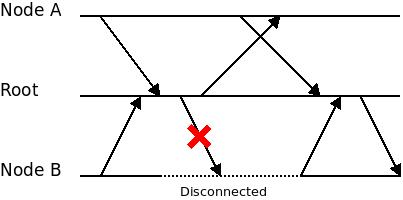
\includegraphics[width=0.6\textwidth]{../images/model_centralized.jpeg}
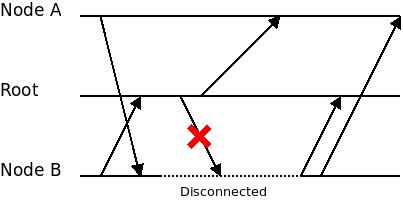
\includegraphics[width=0.6\textwidth]{../images/model_distributed.jpeg}
\caption{Web Delivery Model}
\label{problem_model}
\end{figure}

%What to store
As simple as the model might be, components in it could be vastly heterogenous
while mapping to different techniques. Content stored in a node can either be web objects,
SQL replies, codes or even entire databases. Communication in between can also be
based on a variety of protocols.

%Interactive session
As an online learning platform, users do not only passivly accept information,
but also interact with Moodle through forum, personal blogs and quiz. All the
changes made by users must be stored and seen everywhere. Thus, the system
should not be read-only under any circumstance.

%Dynamic content


%production and minimum affection
Moodle has been in service and adding new services should affect existing
structure as less as possible. Also, steps of adapting changes should be
properly designed to avoid crushing the service.

%communication overhead
To maintain consistency and serve up-to-date content, a reasonable amount of
communication overhead is necessary and is normally positive proportional to the
extent of consistency. Although, due to the presumption of poor network
connection and narrow bandwidth, different nodes in the system are preferably
decoupled and autonomous.

%Offline operation
The autonomy is also closely correlated to the ability of performing offline
operation. Many distributed systems have the ability to detect and recover from
network partitioning, although it normally leads to a compromise of consistensy
and content freshness. When a user request a page, Moodle loads all previliges of the user, generate pages accordingly and log the session. This results in uncacheble content and interaction-must logins.
It has been proven that consistency, high availability and partition tolerence
are impossible to be achieved at same time\cite{brewer2000towards}\cite{gilbert2002brewer}, necessary assumptions must
be made according to the condition and needs.

%Assumptions
While the majority of web caching and content distribution techniques aim at
better performance and delivery efficiency, we prioritize the ability of
performing basic functionalities during network failure. We tolerate a
relatively loose consistency while ensuring eventual convergence.

%Affordability
Lastly, to realize affordability, we mainly focus on open source techniques and
free ware. Thankfully, many successful projects and tools have been made open
source and publicly available. In the following sections of this chapter, we
evaluate a variety of techniques against the criteria stated above and propose
our solution based upon the conclusion. Several of potential solution are also
tried out.

%TODO logic flow chart

\section{Benchmark}

\subsection{Content Delivery Network}
Content Delivery Network overlaps with Web Cache Proxy at the concept of pushing web content to users. A Content Delivery Network is a collaborative set of surrogate servers spanning the network, where web contents are mirrored\cite{pathan2008content}. Users will perceive a smaller latency while fetching content from a nearby CDN surrogate server rather than original web server. The essence of CDN is illustrated in figure X
%TODO figure

Since more and more web services are evolving to provide dynamic content, CDN also takes advantages of cachebility hints when dealing with dynamic contents\cite{dilley2002globally}. 

%TODO open source CDN project

\subsection{Simple Web Caching}
An intuitive and common solution for the problem of limited bandwidth is to cache popular web content locally, as illustrated in Figure \ref{with_cache}.
A server-side web cache proxy typically sits in front of web server, attempting to serve user request with cached objects rather than triggering computational workload on web application. Web caching has been proven to be an effective approach to reduce bandwidth usage, user-perceived latency and loads on original server\cite{davison2001web}.

\begin{figure}[h]
\centering
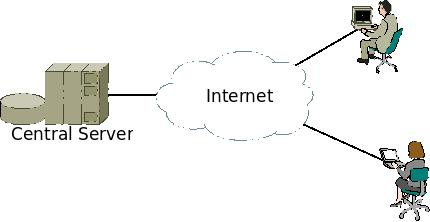
\includegraphics[width=0.6\textwidth]{../images/without_caching.jpeg}
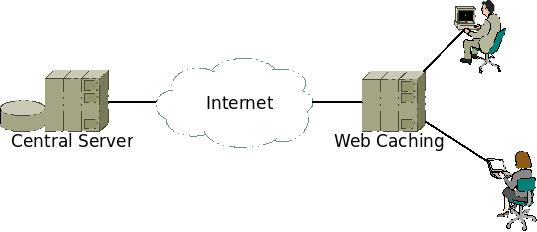
\includegraphics[width=0.6\textwidth]{../images/with_caching.jpeg}
\caption{Serve users without and with a Gateway Cache}
\label{with_cache}
\end{figure}

Web cache is greatly advantageous in our scenario that it does not require modification on web application, except that some TCP optimizations could be done between web cache proxy and web server frontend. Web cache proxy can continue serving requests if offline mode enabled, which also meets our requirements.

Although, all write traffic traverses cache proxy and goes to original server, which leads to a read-only system immediately when network disconnects. This is magnified when Moodle is taken into consideration, where user logins require interaction with original PHP code and database.
%TODO screen shot

%One important feature of all web cache proxies is replacement strategy which invalidate caches and maintain freshness. A comprehensive survey of existing replacement strategy is presented in \cite{podlipnig2003survey}. However

\subsection{Web Caching with Edge Server}
To address the issue of dynamic content generation and client-server interaction, an intuitive and brute-force solution is to replicate application coe, or even the whole website at edge servers\ref{pathan2008content}, see Figure X. In this setup, an edge server is able to act as a complete standalone installation and serve user requests by itself. 


\subsection{Database Replication and Synchronization}

\subsection{Database Cluster}

\section{Multi-Master Database Synchronization}

\subsection{Network File System}
A more brute-force approach is to replicate all three main components in section \ref{components} at local server and have all user requests redirected to it. As a standalone web service, a Moodle installation can be entirely replicated as long as those three components are copied and properly configured.
\subsection{Concurrency Control Protocol}

\subsection{Operational Transformation}
